
\documentclass{beamer}
\usepackage{amsmath}
\usepackage{algorithm}
\usepackage{algpseudocode}
\usepackage{graphicx}
\usepackage{amssymb}
\usepackage{hyperref}

\begin{document}
\title{Hamiltonian Monte Carlo with Graphical Applications}   
\author{Ho Chung Leon Law and Nathan Cunningham} 
\institute[Universities Here and There] % (optional)
{
  OxWaSP 2015 \\
  Department Of Statistics \\
  University Of Oxford\\
}
\date
 {\today}
\frame{\titlepage} 

\section{Section no.1} 
\frame{\frametitle{Hamiltonian Dynamics} 
Hamiltonian dynamics is the system described by a pair of differential equations with coordinates $(\mathbf{q},\mathbf{p}) \in \mathbb{R}^{2d}$.\\ For $i=1 \dots d$,

\begin{equation}
\label{Ham1}
\frac{dq_{i}}{dt} = \frac{\partial H}{\partial p_{i}}
\end{equation}
\begin{equation}
\label{Ham2}
\ \ \frac{dp_{i}}{dt} = -\frac{\partial H}{\partial q_{i}}
\end{equation}
where $H$ is the Hamiltonian and is a function of $(\mathbf{q},\mathbf{p})$.
}
\frame{ \frametitle{Target Density and Energy functions}
From statistical mechanics, given some energy function $E(x)$ in some system, we can express its canonical distribution as:
\begin{equation}
\label{energy}
Pr(x) = \frac{1}{N}\exp(-E(x))
\end{equation}
where $N$ is a normalising constant.
We can rewrite our target density as:
\begin{equation}
U(\mathbf{q}) = -\log [\pi(\mathbf{q})L(\mathbf{q}|D)]
\end{equation}
\\
where $\mathbf{q}\in \mathbb{R}^{d}$ 
\begin{equation}
 P(\mathbf{q})= \pi(\mathbf{q})L(\mathbf{q}|D) \quad \quad q \in \mathbb{R}^{d} 
 \end{equation}
is the target density.
}
\frame{ \frametitle{Construction: Introduction of Auxillary Variable}
Introduce an auxiliary variable $\mathbf{p} \in \mathbb{R}^{d}$ with energy function $K(\mathbf{p})$ and density function $Q(\mathbf{p})$. \\ 
Define the joint density of $(\mathbf{q},\mathbf{p})$:
\begin{equation}
\begin{array}{lcl}
P_{\text{joint}}(\mathbf{q},\mathbf{p}) & = & \frac{1}{Z}\exp(-U(\mathbf{q})/T) \exp(-K(\mathbf{p})/T) \\ \\ &= & \frac{1}{Z}\exp(-H(\mathbf{q},\mathbf{p})/T)
\end{array}
\end{equation}
where $H(\mathbf{q},\mathbf{p}) = U(\mathbf{q}) + K(\mathbf{p})$.  \\
Note $H(\mathbf{q},\mathbf{p})$ the energy function for the joint state $(\mathbf{q},\mathbf{p})$ distribution. }

\frame{\frametitle{Properties of Hamiltonian dynamics}
\begin{itemize}
\item Hamiltonian remains constant.
\item Define $T_s: (\mathbf{q}(t),\mathbf{p}(t)) \rightarrow (\mathbf{q}(t+s),\mathbf{p}(t+s))$,  the arrow represents the evolution of the dynamics. The mapping $T_s$ is reversible.
\item Hamiltonian dynamics preserves volume in the $(\mathbf{q},\mathbf{p})$ space, i.e. the image of $T_s$ from some region R has the same volume as region R.
\end{itemize} 
}

\frame{\frametitle{Hamiltonian Dynamics and Hamiltonian Monte Carlo}
Idea: Construct a Hamiltonian and Markov chain that make use of these properties. \\
Illustration:
$U(q)=\dfrac{q^2}{2}$ \\
Transfer of `Energy' between $U(q)$ and $P(q)$ after giving particle some random momentum, a normal is commonly used.
\begin{figure}[H]
\center
  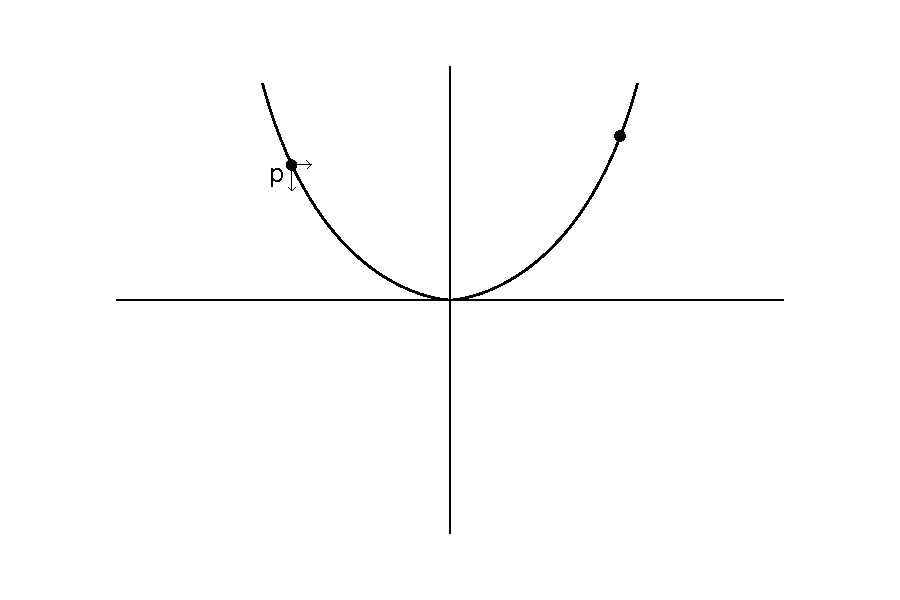
\includegraphics[width=3.7in]{images/momentum.pdf}
\end{figure}
}
\frame{\frametitle{The `Ideal' Algorithm}
\begin{enumerate}
\item initial $\mathbf{q}$
\item $\mathbf{p}\sim \mathcal{MN}(\mathbf{0},\mathbf{M})$
\item Given $(\mathbf{q},\mathbf{p})$, simulate Hamiltonian dynamics for some time and obtain $(\mathbf{q^{*}}, \mathbf{p^{*}})$.
\item Negate $\mathbf{p^{*}}$ to ensure reversibility.
\item Accept $(\mathbf{q^{*}}, \mathbf{p^{*}})$ as the next step in the Markov chain with probability 1.
\end{enumerate}
\begin{figure}[H]
\center
  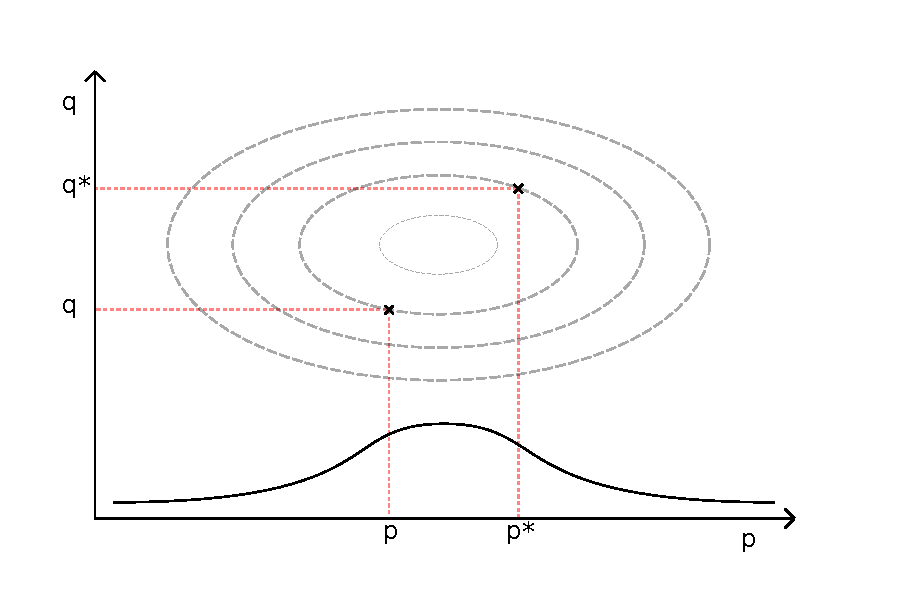
\includegraphics[width=3in]{images/contours.pdf}
\end{figure}
 }
\frame{\frametitle{World is not ideal: LeapFrog}
Can not solve analytically. S: Discretize and pick $L$ and $\epsilon$.
\begin{equation}
p_{i}(t+\epsilon/2) = p_{i}(t) - (\epsilon/2)\frac{\partial U}{\partial q_{i}}(\mathbf{q}(t))
\end{equation}
\begin{equation}
q_{i}(t+\epsilon) = q_{i}(t) - (\epsilon)\frac{p_{i}(t+\epsilon/2)}{m_{i}}
\end{equation}
\begin{equation}
p_{i}(t+\epsilon) = p_{i}(t+\epsilon/2) - (\epsilon/2)\frac{\partial U}{\partial q_{i}}(\mathbf{q}(t+\epsilon))
\end{equation}
Iterating over this process $L$ times simulates the dynamics for a time of $L\epsilon$.
}
\frame{\frametitle{HMC Algorithm}
Use Metropolis to correct the approximation error made in Leapfrog.
\begin{enumerate}
\item  Select an initial $\mathbf{q}$.
\item $\mathbf{p}\sim \mathcal{MN}(\mathbf{0},\mathbf{M})$
\item  Given $(\mathbf{q},\mathbf{p})$, simulate Hamiltonian dynamics using the leapfrog for $L$ steps with $\epsilon$ to find $(\mathbf{q^{*}},\mathbf{p^{*}})$.
\item Negate $\mathbf{p^{*}}$ to ensure reversibility.
\item Accept $(\mathbf{q^{*}}, \mathbf{p^{*}})$ as the next step in the Markov chain with probability M given below, otherwise accept $(\mathbf{q},\mathbf{p})$ as next state.
\end{enumerate}
\begin{equation}
\begin{array}{lcl}
M &=&\min \{1,\exp(-H(\mathbf{q^{*}},\mathbf{p^{*}})+H(\mathbf{q},\mathbf{p}))\} \\ &=& \min\{1, \exp(-U(\mathbf{q^{*}})+U(\mathbf{q})-K(\mathbf{p^{*}})+K(\mathbf{p}))\}
\end{array}
\end{equation}
}

\frame{\frametitle{Comparison between HMC and MH}
\begin{itemize}
\item 25 samples simulated from a bivariate Gaussian with marginal mean $0$, $\sigma = 1$ and correlation of $0.95$
\item HMC: $\epsilon = 0.20$ and $L = 25$  Rejection Rate$=0$
\item MH: uniform proposal with $U[-0.25,0.25]$ around the current state with thinning of 25 samples. Rejection Rate$=0.5$.
\end{itemize}
\begin{figure}[H]
\center
  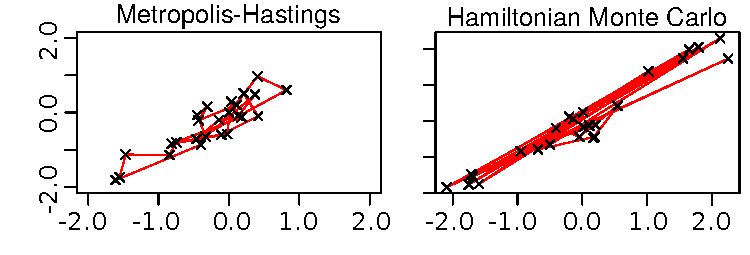
\includegraphics[width=4in]{images/MHvsHM_explore.pdf}
\end{figure}
}
\frame{\frametitle{Multivariate Gaussian (150 dimensions): HMC, MH}
\begin{itemize}
\item 1000 samples from a 150-dimensional independent Gaussian with increasing variance.
\item HMC: $\epsilon=0.014$ and $L=100$. Rejection Rate$=0.05$.
\item MH: uniform proposal with $U[-0.02,0.02]$ around the current state with thinning of 60 samples.
\end{itemize}
\begin{figure}[H]
\center
  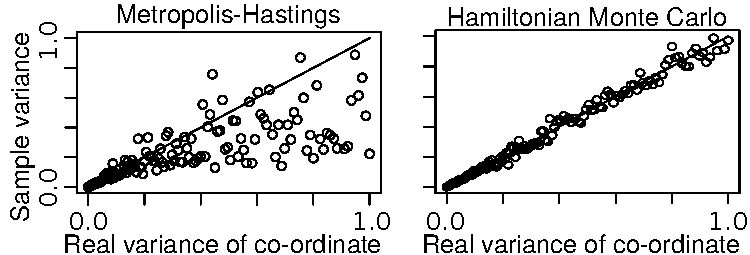
\includegraphics[width=4in]{images/MHvsHM_varcoord.pdf}
\end{figure}

}

\frame{\frametitle{NUTS}
\begin{itemize}
\item No U-Turn sampling modelled through $RStan$ package
\item 150-dimensional Gaussian simulated over 1000 samples
\end{itemize}
\begin{figure}[H]
\center
  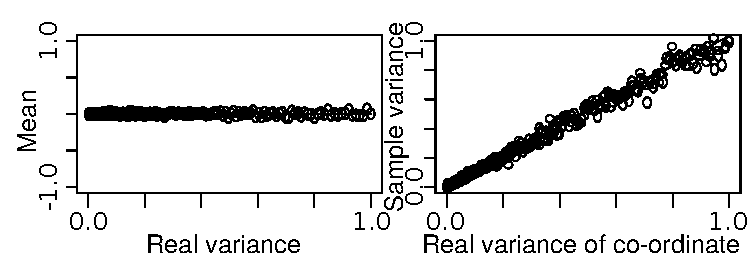
\includegraphics[width=4in]{images/NUTS_comparisons.pdf}
\end{figure}

}

\frame{\frametitle{Graphical presentation: abcHMC}
\begin{itemize}
\item Simulate samples from 2 bivariate Gaussian mixtures whose densities represent the letters of the alphabet
\item Mixture models fitted automatically using EM algorithm and an image dataset for 52 letters and `!' and `?'.
\item Equal weighting on each letter of a word.
\item Simulate from the samples using using HMC and MH.
\item abcHMC package can be found on Github.
\end{itemize}
}

\end{document}